\Lecture{Dinesh K.}{Mar 6, 2012}{35}{Size and Depth complexity of Boolean Circuits}

%\theme{Circuit Complexity}
%\lectureplan{ Notion of size and depth of circuits. Shannon's and 
%Lupanov's bound on size of circuits computing any boolean function.}

In the previous lecture, we saw what boolean functions, family of 
boolean functions are, defined function computation and argued that boolean 
circuits are natural notions for computing boolean functions. We also saw the 
notion of complete basis and characterisation of complete basis due Emil Post.

In this lecture, we shall see two important parameters of a circuit called 
\emph{size complexity} and \emph{depth complexity} and shall look into 
Lupanov's (upper) bound and Shannon's (lower) bound on the size of a circuit
computing a function.

Before delving deep, let's have a look at the following definitions.

\section{Definitions}
\begin{definition}(Family of circuits) Let $\{C_n\}_{n \ge 0}$ be an infinite
collection where each $c_i$ is a boolean circuit (computing a boolean
function) on the $i$ input lines.
\end{definition}
This definition is similar to our notion of family of functions defined in
the previous lecture.

\begin{definition}
Let $L \subseteq \Sigma^*$, $x \in \Sigma^*$. Let the characteristic function
of $L$ on inputs of length $n$ be defined as ,
\[
\chi_L^{(n)}(x) = 
	\begin{cases}
	1 & \text{if } x \in L \cap \{0,1\}^n, \\
	0 & \text{otherwise}
	\end{cases}
\]
\end{definition}

\begin{definition}
$L \subseteq \Sigma^*$ is computed \footnote{When we say $L$ is computed by a
circuit family, we do not worry about how to get the circuit family. The
issue of whether the family exists or not shall be addressed in the
subsequent lectures.} by a family of circuits if $\exists \{C_n\}_{n \ge 0}$
such that \[ x \in L \iff C_{|x|}(x) = 1 \]
Essentially $C_n$ computes the function $\chi_L^{(n)}(x)$
\end{definition}
Observe that the circuit computing a function on $n$ input can be
drastically different from a circuit computing the same function on $n+1$
inputs. This leads to the notion of \emph{non-uniform} computation which can
be stated informally as the case where there is no single circuit that
decides the language, yet for strings of the same length there is a single
device (circuit) that decides them.

\section{Parameters of Interest}
To understand what parameters of circuit are we interested in, let us try
to gain some motivation from the parallel computation world. In parallel
computation, the aim is to decompose the jobs and then each job is processed
by one processor. 
\begin{figure}[htp!]
\centering
\begin{picture}(0,0)%
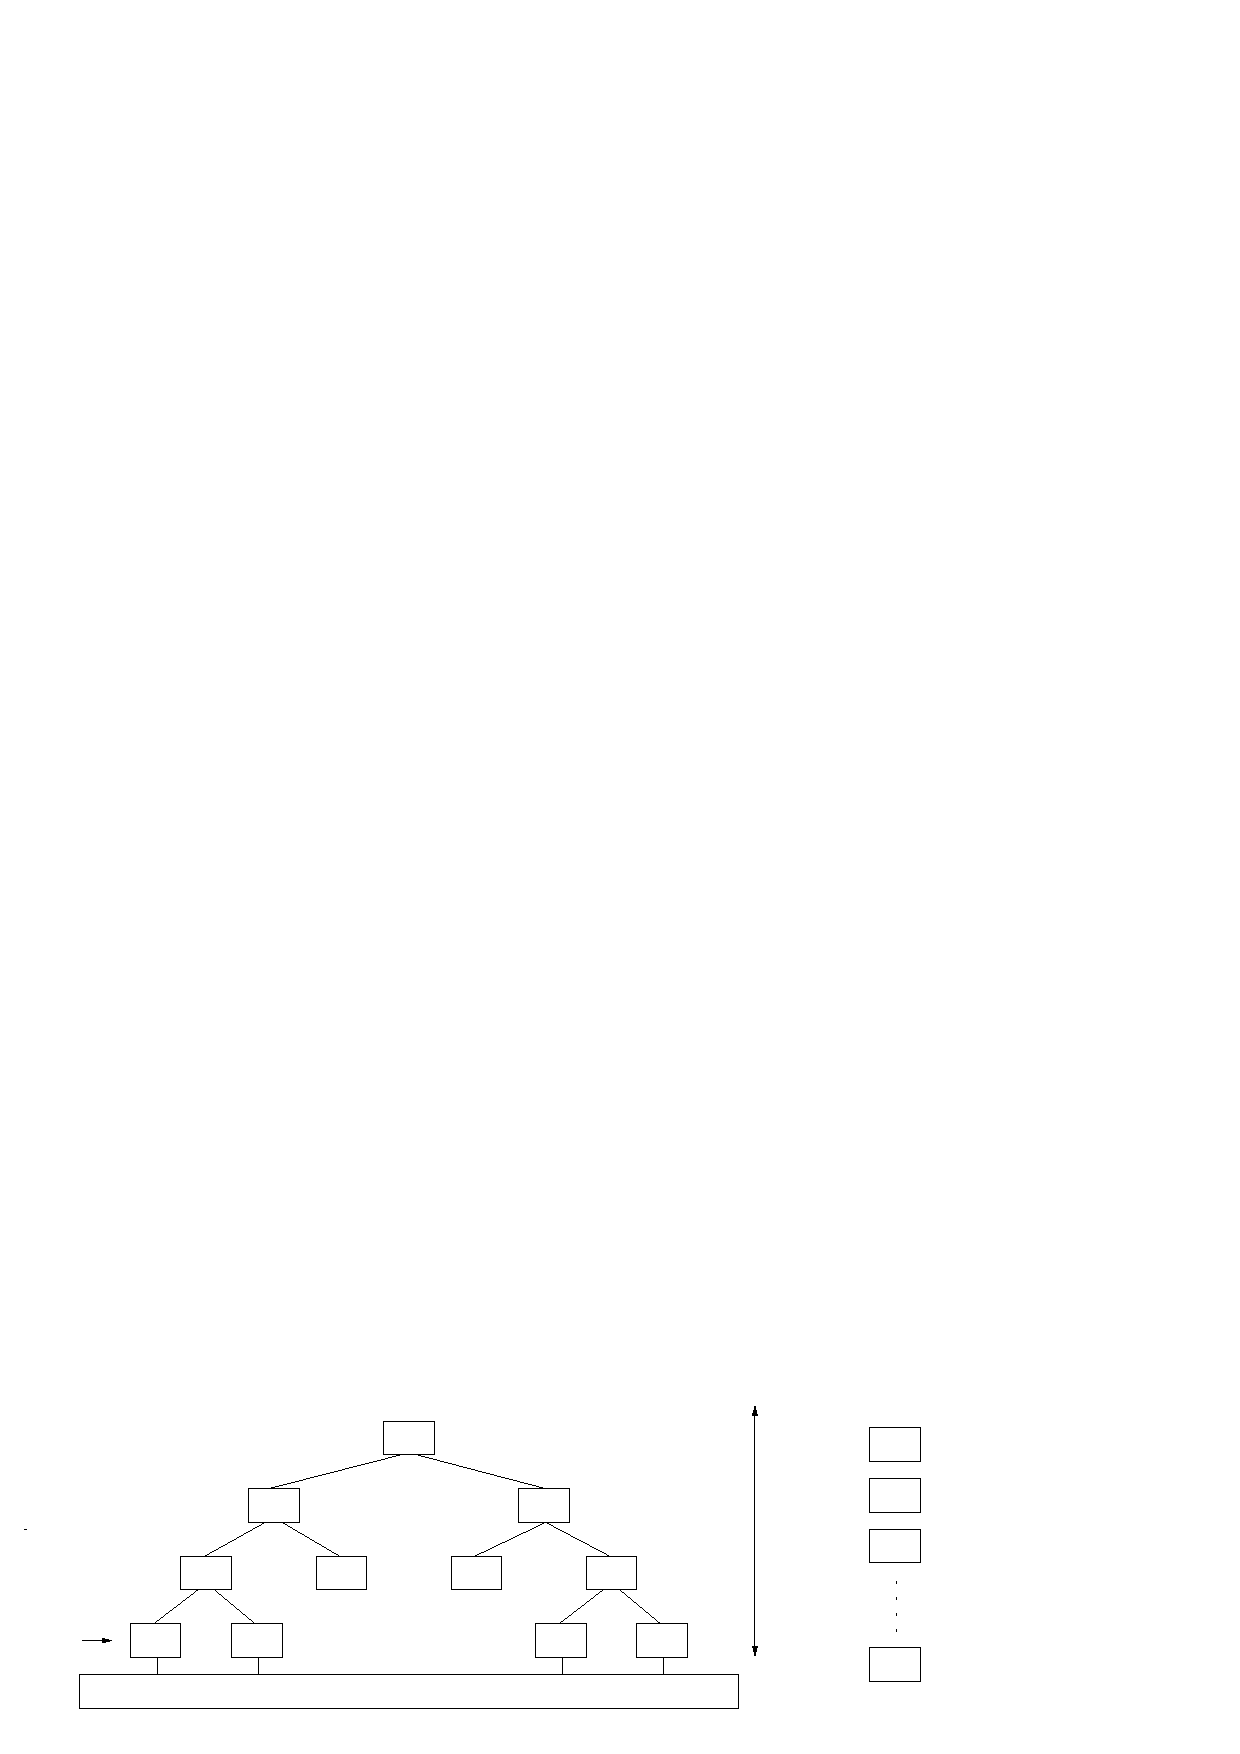
\includegraphics{Lecture35-Dinesh/figs/fig1.pdf}%
\end{picture}%
\setlength{\unitlength}{4144sp}%
%
\begingroup\makeatletter\ifx\SetFigFont\undefined%
\gdef\SetFigFont#1#2#3#4#5{%
  \reset@font\fontsize{#1}{#2pt}%
  \fontfamily{#3}\fontseries{#4}\fontshape{#5}%
  \selectfont}%
\fi\endgroup%
\begin{picture}(7191,2676)(3631,-7990)
\put(10183,-7942){\makebox(0,0)[lb]{\smash{{\SetFigFont{7}{8.4}{\rmdefault}{\mddefault}{\updefault}{\color[rgb]{0,0,0}computation}%
}}}}
\put(10183,-7796){\makebox(0,0)[lb]{\smash{{\SetFigFont{7}{8.4}{\rmdefault}{\mddefault}{\updefault}{\color[rgb]{0,0,0}Sequential}%
}}}}
\put(9463,-7539){\makebox(0,0)[lb]{\smash{{\SetFigFont{7}{8.4}{\rmdefault}{\mddefault}{\updefault}{\color[rgb]{0,0,0}Input}%
}}}}
\put(9463,-6304){\makebox(0,0)[lb]{\smash{{\SetFigFont{7}{8.4}{\rmdefault}{\mddefault}{\updefault}{\color[rgb]{0,0,0}depth}%
}}}}
\put(3646,-7153){\makebox(0,0)[lb]{\smash{{\SetFigFont{7}{8.4}{\rmdefault}{\mddefault}{\updefault}{\color[rgb]{0,0,0}Processors}%
}}}}
\put(5859,-7847){\makebox(0,0)[lb]{\smash{{\SetFigFont{7}{8.4}{\rmdefault}{\mddefault}{\updefault}{\color[rgb]{0,0,0}Parallel job computation}%
}}}}
\end{picture}%

\caption{Parallel and Sequential computation}
\label{figure1}
\end{figure}

But there can be parallelism in the outcomes of these processors. So we again
have a processors that receives the processed input and carry on the
processing (figure~\ref{figure1}) thereby leading levels of computation. 
In case of sequential computation, no such decomposition is possible : 
each processor in the same level will be executed one after the other and will 
be repeated for all the levels.

What would be the ``parallel'' time taken to finish the job ? This is nothing
but the time required to get the output. Since input to each level is
dependent on the output of the previous level, the delay caused will be
proportional to the length of the longest path.

Circuits essentially tries to abstract this idea.
\begin{definition}(Depth) Depth of any circuit $C$ is a function $\calD$ that
takes in circuit and gives the length of the longest path from root 
(output) to any leaf (input).
\end{definition}

\begin{definition}(Size) Size of a circuit $C$ is a function $\calS$ 
that takes a circuit and gives the number of gates (or devices) in the circuit.

Note that the size of a circuit can also be thought as the time taken by a
sequential machine to compute the same function.
\end{definition}

\begin{example}
Consider the parity function $f : \{0,1\}^n \to \{0,1\}$ where
$f(x_1,x_2,\ldots,x_n) = x_1 \oplus x_2 \oplus \ldots \oplus x_n$. The
circuit corresponding to this function is as shown in figure~\ref{figure2}.

\begin{figure}[htp!]
\centering
\begin{picture}(0,0)%
\includegraphics{Lecture35-Dinesh/figs/fig2.pdf}%
\end{picture}%
\setlength{\unitlength}{4144sp}%
%
\begingroup\makeatletter\ifx\SetFigFont\undefined%
\gdef\SetFigFont#1#2#3#4#5{%
  \reset@font\fontsize{#1}{#2pt}%
  \fontfamily{#3}\fontseries{#4}\fontshape{#5}%
  \selectfont}%
\fi\endgroup%
\begin{picture}(4702,1911)(886,-2197)
\put(5004,-2151){\makebox(0,0)[lb]{\smash{{\SetFigFont{7}{8.4}{\rmdefault}{\mddefault}{\updefault}{\color[rgb]{0,0,0}$x_{n-1}$}%
}}}}
\put(5452,-2151){\makebox(0,0)[lb]{\smash{{\SetFigFont{7}{8.4}{\rmdefault}{\mddefault}{\updefault}{\color[rgb]{0,0,0}$x_n$}%
}}}}
\put(1349,-2151){\makebox(0,0)[lb]{\smash{{\SetFigFont{7}{8.4}{\rmdefault}{\mddefault}{\updefault}{\color[rgb]{0,0,0}$x_2$}%
}}}}
\put(901,-2151){\makebox(0,0)[lb]{\smash{{\SetFigFont{7}{8.4}{\rmdefault}{\mddefault}{\updefault}{\color[rgb]{0,0,0}$x_1$}%
}}}}
\put(2443,-2151){\makebox(0,0)[lb]{\smash{{\SetFigFont{7}{8.4}{\rmdefault}{\mddefault}{\updefault}{\color[rgb]{0,0,0}$x_3$}%
}}}}
\put(2890,-2151){\makebox(0,0)[lb]{\smash{{\SetFigFont{7}{8.4}{\rmdefault}{\mddefault}{\updefault}{\color[rgb]{0,0,0}$x_4$}%
}}}}
\put(3164,-485){\makebox(0,0)[lb]{\smash{{\SetFigFont{7}{8.4}{\rmdefault}{\mddefault}{\updefault}{\color[rgb]{0,0,0}$+$}%
}}}}
\put(4457,-1231){\makebox(0,0)[lb]{\smash{{\SetFigFont{7}{8.4}{\rmdefault}{\mddefault}{\updefault}{\color[rgb]{0,0,0}$+$}%
}}}}
\put(5253,-1728){\makebox(0,0)[lb]{\smash{{\SetFigFont{7}{8.4}{\rmdefault}{\mddefault}{\updefault}{\color[rgb]{0,0,0}$+$}%
}}}}
\put(3711,-1728){\makebox(0,0)[lb]{\smash{{\SetFigFont{7}{8.4}{\rmdefault}{\mddefault}{\updefault}{\color[rgb]{0,0,0}$+$}%
}}}}
\put(2691,-1728){\makebox(0,0)[lb]{\smash{{\SetFigFont{7}{8.4}{\rmdefault}{\mddefault}{\updefault}{\color[rgb]{0,0,0}$+$}%
}}}}
\put(1896,-1231){\makebox(0,0)[lb]{\smash{{\SetFigFont{7}{8.4}{\rmdefault}{\mddefault}{\updefault}{\color[rgb]{0,0,0}$+$}%
}}}}
\put(1171,-1726){\makebox(0,0)[lb]{\smash{{\SetFigFont{7}{8.4}{\rmdefault}{\mddefault}{\updefault}{\color[rgb]{0,0,0}$+$}%
}}}}
\end{picture}%

\caption{The parity function}
\label{figure2}
\end{figure}
Note that we have exploited the associativity property of $\oplus$.
This circuit has a size $= n-1$ and depth $=\lceil\log_2 n \rceil$.
\end{example}

The next natural question to ask is 
\begin{center}
Will the parameters $\calS$ and $\calD$ depend on the complete basis chosen ?
\end{center}
The answer is yes and we now give a more accurate definition of size and
depth in terms of languages.
\begin{definition}Size $S_\Omega(L)$ of a language $L$ is the minimum
sized\footnote{By minimum sized, we mean asymptotic size i.e. constant
factors are ignored} function of a circuit family that computes $L$ for the
complete basis $\Omega$.
\end{definition}
\begin{definition}Depth $D_\Omega(L)$ of a language $L$ is the minimum
depth function of a circuit family that computes $L$ for the
complete basis $\Omega$.
\end{definition}

\begin{definition}Circuit Complexity of a language $L$ for a complete basis
$\Omega$ is defined as the tuple $(\calS_\Omega(L), \calD_\Omega(L))$ which
corresponds to the size and depth complexities respectively.
\end{definition}

\begin{claim}
\label{basis}
Let $\Omega$, $\Omega'$ be two finite complete basis of boolean functions of
fixed arity. Then for any $L \in \Sigma^*$,
\[ \calS_\Omega(L) = \Theta(\calS_{\Omega'}(L)), 
 \calD_\Omega(L) = \Theta(\calD_{\Omega'}(L)) \] 
\end{claim}
\begin{proof-idea}
Let $\{C_n\}_{n \ge 0}$ be the minimum sized circuit computing $L$ for the
complete basis $\Omega$. When the basis is changed, one need to express
boolean functions in $\Omega$ in terms of boolean functions in $\Omega'$.
This is always possible since $\Omega'$ is complete. Now a circuit in
the basis $\Omega'$ can be obtained by replacing the gates in $\Omega$ by
their equivalent circuits in $\Omega'$.

Note that the basis is finite and is independent of $n$. So the blow up or
shrinkage of each gate $C_n$ will only be by a constant. Hence in the worst
case all the gates in $\{C_n\}$ gets scaled by a constant factor and the size
of the resultant circuit can be at most $k \times$ size of original circuit. 
In case of depth, the length of the longest path gets scaled up (or down) by 
a factor independent of $n$.
\end{proof-idea}


Now we define the complexity class corresponding to the circuits computing a
function.
\begin{definition} For functions $f,g : \N \to \N$
\begin{align*}
SIZE(f(n)) & = \{ L | L \text{ is computed by a family of circuits of size }
f(n) \} \\
DEPTH(g(n)) & = \{ L | L \text{ is computed by a family of circuits of depth }
g(n) \} 
\end{align*}
\end{definition}

\section{Size of Circuits computing Boolean functions}
Consider a boolean function $f: \{0,1\}^n \to \{0,1\}$ defined on the
variables $(x_1,x_2,\ldots,x_n) \in \{0,1\}^n$ and the complete basis
$\Omega = \{\land,\lor,\neg\}$ where each function is having an arity $2$.
By claim~\ref{basis}, we have already seen that fixing the basis to be finite
gives us the guarantee that the same result holds in other bases
asymptotically. From now on we shall be working on this complete basis.

We would like to know what would be the size of the circuit computing $f$. How
large or small can it be ? Before answering them let us see what would be the
trivial circuit computing $f$.

An easy way to look at $f$ is to express it as sum-of-product terms (which can
be figured out from the truth table of $f$). Hence 
\[ f(x_1,x_2,\ldots,x_n) = \bigvee_{f(a_1,a_2,\ldots,a_n) = 1}(x_1^{a_1} \land
x_2^{a_2} \land \ldots \land x_n^{a_n} ) \]
where,
\[ x_i^{a_i} = \begin{cases}
		\overline{x_i} & \text{if } a_i = 0, \\
		x_i & \text{if } a_i = 1
		\end{cases} \]
\pagebreak

A circuit representation of $f$ (shown in figure~\ref{figure3})
\begin{figure}[htp!]
\centering
\begin{picture}(0,0)%
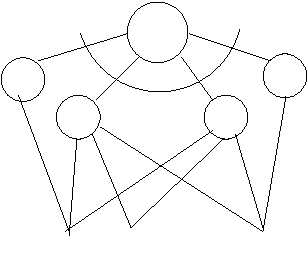
\includegraphics{Lecture35-Dinesh/figs/fig3.pdf}%
\end{picture}%
\setlength{\unitlength}{4144sp}%
%
\begingroup\makeatletter\ifx\SetFigFont\undefined%
\gdef\SetFigFont#1#2#3#4#5{%
  \reset@font\fontsize{#1}{#2pt}%
  \fontfamily{#3}\fontseries{#4}\fontshape{#5}%
  \selectfont}%
\fi\endgroup%
\begin{picture}(2347,1973)(3246,-3010)
\put(3624,-2912){\makebox(0,0)[lb]{\smash{{\SetFigFont{8}{9.6}{\familydefault}{\mddefault}{\updefault}{\color[rgb]{0,0,0}$x_1$}%
}}}}
\put(4097,-2912){\makebox(0,0)[lb]{\smash{{\SetFigFont{8}{9.6}{\familydefault}{\mddefault}{\updefault}{\color[rgb]{0,0,0}$x_2$}%
}}}}
\put(5100,-2912){\makebox(0,0)[lb]{\smash{{\SetFigFont{8}{9.6}{\familydefault}{\mddefault}{\updefault}{\color[rgb]{0,0,0}$x_n$}%
}}}}
\put(5130,-1228){\makebox(0,0)[lb]{\smash{{\SetFigFont{8}{9.6}{\rmdefault}{\mddefault}{\updefault}{\color[rgb]{0,0,0}$2^n$}%
}}}}
\put(3376,-1681){\makebox(0,0)[lb]{\smash{{\SetFigFont{8}{9.6}{\familydefault}{\mddefault}{\updefault}{\color[rgb]{0,0,0}$\land$}%
}}}}
\put(3826,-1951){\makebox(0,0)[lb]{\smash{{\SetFigFont{8}{9.6}{\familydefault}{\mddefault}{\updefault}{\color[rgb]{0,0,0}$\land$}%
}}}}
\put(4951,-1951){\makebox(0,0)[lb]{\smash{{\SetFigFont{8}{9.6}{\familydefault}{\mddefault}{\updefault}{\color[rgb]{0,0,0}$\land$}%
}}}}
\put(5401,-1636){\makebox(0,0)[lb]{\smash{{\SetFigFont{8}{9.6}{\familydefault}{\mddefault}{\updefault}{\color[rgb]{0,0,0}$\land$}%
}}}}
\put(4411,-1321){\makebox(0,0)[lb]{\smash{{\SetFigFont{12}{14.4}{\familydefault}{\mddefault}{\updefault}{\color[rgb]{0,0,0}$\vee$}%
}}}}
\put(4366,-2041){\makebox(0,0)[lb]{\smash{{\SetFigFont{12}{14.4}{\rmdefault}{\mddefault}{\updefault}{\color[rgb]{0,0,0}$\ldots$}%
}}}}
\put(4546,-2941){\makebox(0,0)[lb]{\smash{{\SetFigFont{12}{14.4}{\rmdefault}{\mddefault}{\updefault}{\color[rgb]{0,0,0}$\ldots$}%
}}}}
\end{picture}%

\caption{Circuit representation of $f$}
\label{figure3}
\end{figure}
has a root $\vee$ gate with $2^n$ inputs. But our basis has $\lor$ gates of 
arity $2$. Reduction to arity $2$ can be achieved by composing $\lor$ as shown.
in figure~\ref{figure4}
\begin{figure}[htp!]
\centering
\begin{picture}(0,0)%
\includegraphics{Lecture35-Dinesh/figs/fig4.pdf}%
\end{picture}%
\setlength{\unitlength}{4144sp}%
%
\begingroup\makeatletter\ifx\SetFigFont\undefined%
\gdef\SetFigFont#1#2#3#4#5{%
  \reset@font\fontsize{#1}{#2pt}%
  \fontfamily{#3}\fontseries{#4}\fontshape{#5}%
  \selectfont}%
\fi\endgroup%
\begin{picture}(2271,2451)(1789,-3175)
\put(4045,-1638){\makebox(0,0)[lb]{\smash{{\SetFigFont{5}{6.0}{\rmdefault}{\mddefault}{\updefault}{\color[rgb]{0,0,0}depth $n$}%
}}}}
\put(3408,-1749){\makebox(0,0)[lb]{\smash{{\SetFigFont{5}{6.0}{\rmdefault}{\mddefault}{\updefault}{\color[rgb]{0,0,0}$\lor$}%
}}}}
\put(3166,-1352){\makebox(0,0)[lb]{\smash{{\SetFigFont{5}{6.0}{\rmdefault}{\mddefault}{\updefault}{\color[rgb]{0,0,0}$\lor$}%
}}}}
\put(2725,-957){\makebox(0,0)[lb]{\smash{{\SetFigFont{5}{6.0}{\rmdefault}{\mddefault}{\updefault}{\color[rgb]{0,0,0}$\lor$}%
}}}}
\put(2351,-1352){\makebox(0,0)[lb]{\smash{{\SetFigFont{5}{6.0}{\rmdefault}{\mddefault}{\updefault}{\color[rgb]{0,0,0}$\lor$}%
}}}}
\put(2548,-1771){\makebox(0,0)[lb]{\smash{{\SetFigFont{5}{6.0}{\rmdefault}{\mddefault}{\updefault}{\color[rgb]{0,0,0}$\lor$}%
}}}}
\put(2637,-3136){\makebox(0,0)[lb]{\smash{{\SetFigFont{5}{6.0}{\rmdefault}{\mddefault}{\updefault}{\color[rgb]{0,0,0}$2^n$ inputs}%
}}}}
\put(2109,-1749){\makebox(0,0)[lb]{\smash{{\SetFigFont{5}{6.0}{\rmdefault}{\mddefault}{\updefault}{\color[rgb]{0,0,0}$\lor$}%
}}}}
\put(2945,-1749){\makebox(0,0)[lb]{\smash{{\SetFigFont{5}{6.0}{\rmdefault}{\mddefault}{\updefault}{\color[rgb]{0,0,0}$\lor$}%
}}}}
\end{picture}%

\caption{Arity reduction of root $\lor$ gate}
\label{figure4}
\end{figure}
and replacing the root $\lor$ gate in figure~\ref{figure3} by this circuit. 
Again the $\land$ gates are taking $n$ inputs: hence we replace the $\land$ 
gate by composing $\land$ s as shown in figure~\ref{figure5} 
and plug it in place of $\land$ in figure~\ref{figure3}.

\begin{figure}[htp!]
\centering
\begin{picture}(0,0)%
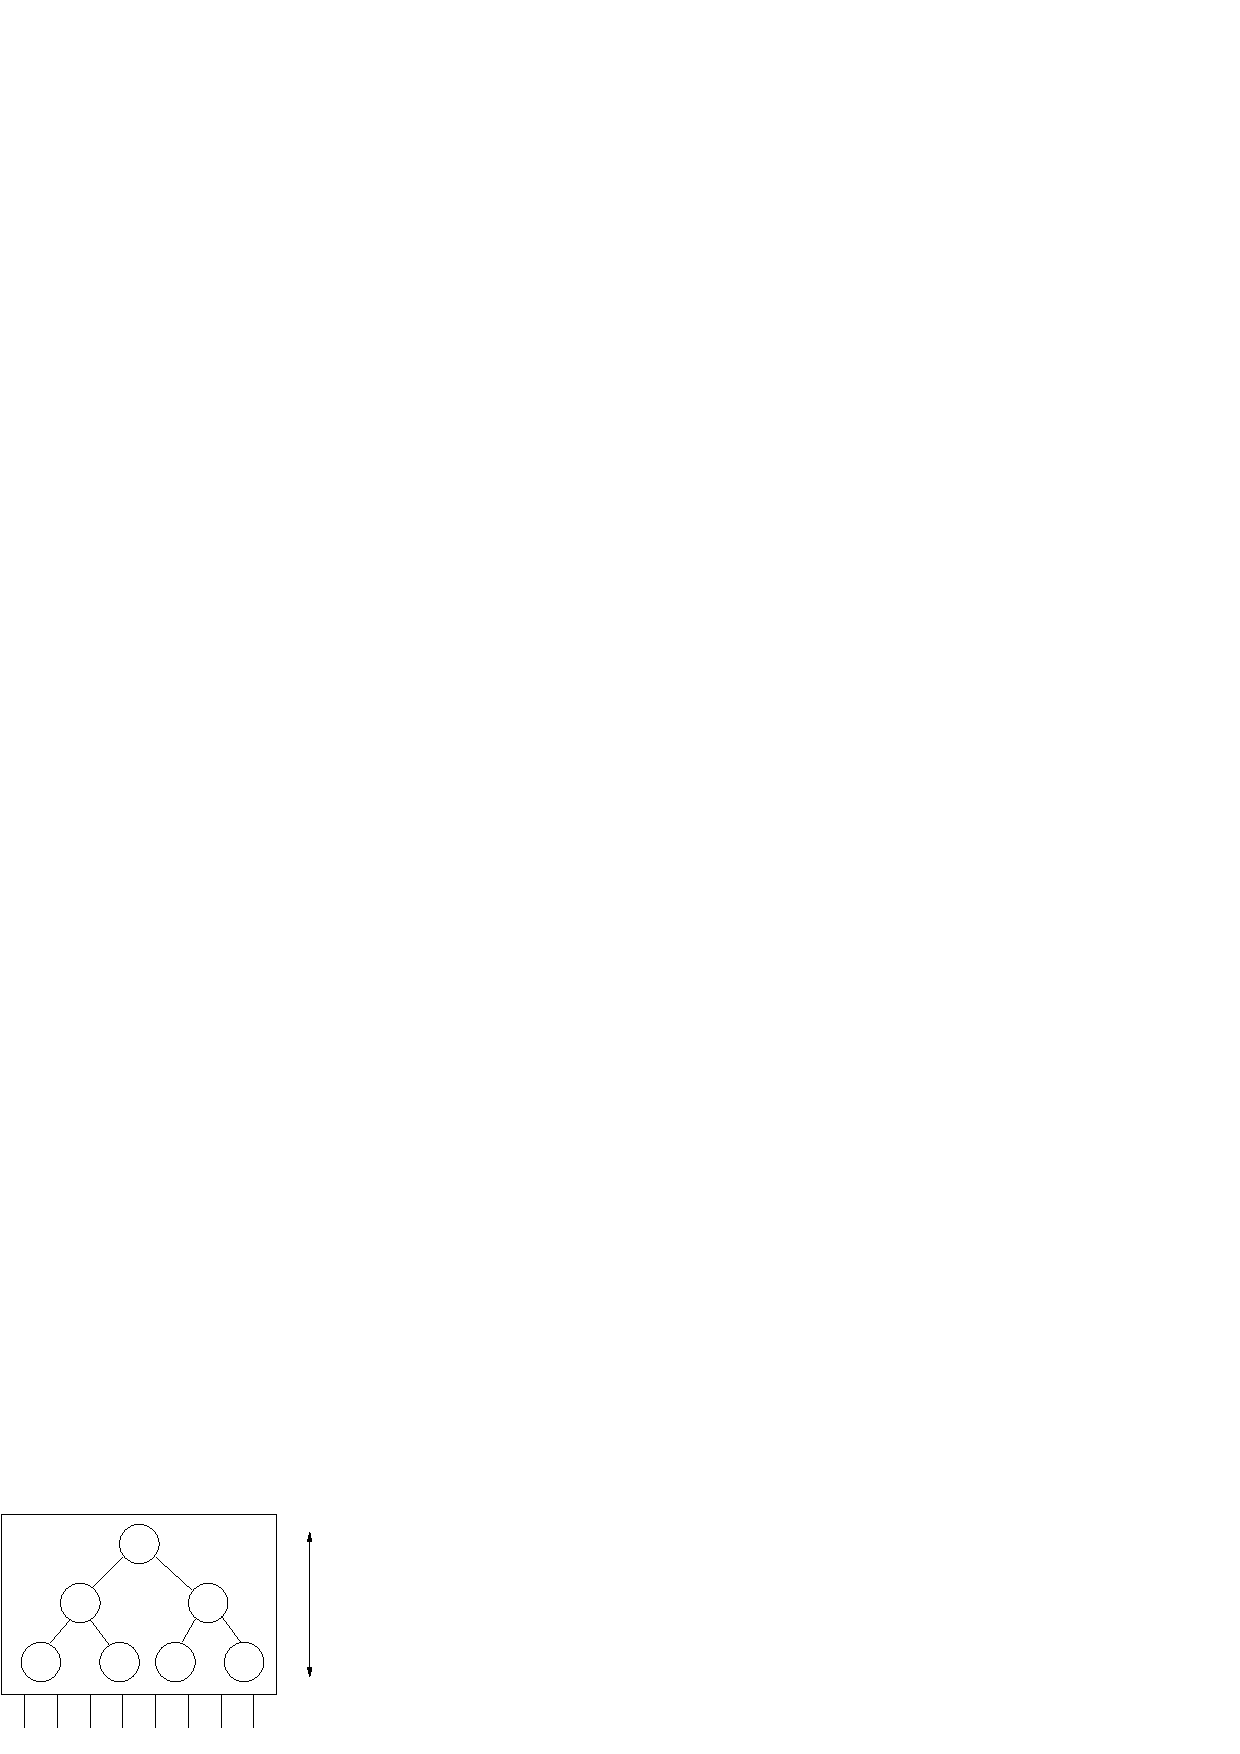
\includegraphics{Lecture35-Dinesh/figs/fig5.pdf}%
\end{picture}%
\setlength{\unitlength}{4144sp}%
%
\begingroup\makeatletter\ifx\SetFigFont\undefined%
\gdef\SetFigFont#1#2#3#4#5{%
  \reset@font\fontsize{#1}{#2pt}%
  \fontfamily{#3}\fontseries{#4}\fontshape{#5}%
  \selectfont}%
\fi\endgroup%
\begin{picture}(2401,1837)(1834,-2561)
\put(2021,-1886){\makebox(0,0)[lb]{\smash{{\SetFigFont{7}{8.4}{\familydefault}{\mddefault}{\updefault}{\color[rgb]{0,0,0}$\land$}%
}}}}
\put(2321,-1436){\makebox(0,0)[lb]{\smash{{\SetFigFont{7}{8.4}{\rmdefault}{\mddefault}{\updefault}{\color[rgb]{0,0,0}$\land$}%
}}}}
\put(2621,-1886){\makebox(0,0)[lb]{\smash{{\SetFigFont{7}{8.4}{\familydefault}{\mddefault}{\updefault}{\color[rgb]{0,0,0}$\land$}%
}}}}
\put(3046,-1886){\makebox(0,0)[lb]{\smash{{\SetFigFont{7}{8.4}{\familydefault}{\mddefault}{\updefault}{\color[rgb]{0,0,0}$\land$}%
}}}}
\put(3296,-1436){\makebox(0,0)[lb]{\smash{{\SetFigFont{7}{8.4}{\familydefault}{\mddefault}{\updefault}{\color[rgb]{0,0,0}$\land$}%
}}}}
\put(2771,-986){\makebox(0,0)[lb]{\smash{{\SetFigFont{7}{8.4}{\familydefault}{\mddefault}{\updefault}{\color[rgb]{0,0,0}$\land$}%
}}}}
\put(3571,-1886){\makebox(0,0)[lb]{\smash{{\SetFigFont{7}{8.4}{\familydefault}{\mddefault}{\updefault}{\color[rgb]{0,0,0}$\land$}%
}}}}
\put(2671,-2511){\makebox(0,0)[lb]{\smash{{\SetFigFont{7}{8.4}{\familydefault}{\mddefault}{\updefault}{\color[rgb]{0,0,0}$n$ inputs}%
}}}}
\put(4220,-1486){\makebox(0,0)[lb]{\smash{{\SetFigFont{7}{8.4}{\familydefault}{\mddefault}{\updefault}{\color[rgb]{0,0,0}depth $\lceil \log n \rceil$}%
}}}}
\end{picture}%

\caption{Arity reduction of $\land$ gate}
\label{figure5}
\end{figure}

Now size of the circuit 
\begin{align*}
= &   (2^{n+1}-1)  && \text{[due to $\lor$ gates]} \\ 
  & + 2^n \times (2n-1) && \text{[due to $2^n$ $\land$ 
  gates each of size $(2n-1)$]} \\
  =&  O(n 2^n) 
\end{align*}

A takeaway from the whole exercise is that any function $f$ on $n$ input can
be represented using a circuit of size $O(n2^n)$.
A natural question is : can there be circuits of even smaller size ?

We shall now see a lower bound due to Shannon(1942) and an upper bound due to
Lupanov(1952) on the size of a boolean circuit computing a function $f$.

\section{Shannon's Lower bound}
\begin{theorem}(Shannon, 1942) For  ``most'' of the circuits on $n$ inputs
computing a function $f$, the size of the circuit is larger than
$\frac{2^n}{n}$ (asymptotically)
\end{theorem}
\begin{proof}
Proof is by a counting argument on the number of boolean circuits on $n$
inputs and of size $s$ computing $f$. We argue that if we restrict the size of
the circuit $s < \frac{2^n}{n}$, then the fraction of functions that can be
computed using such circuits is very small.

Let $H(n,s)$ be the number of distinct circuits possible on $n$ inputs and of
size $s$. Observe that $s \ge n$. Since the circuit is characterised by a
(unique) root, $s-1$ gates and $n$ inputs, we count how many ways can the $s$
gates be \emph{selected}. The count can be split as,
\begin{itemize}
\item No. of ways of fixing the root $\to$ $s$ ways.
\item Each of the internal gates (gates other than the root)
   \begin{itemize}
   \item can compute $2^{2^2}$ functions\footnote{$\neg$ can be assumed to be
   of two input where it negates one input and ignores the other.}
   \item there are $(n+s)$ possible inputs for each function and hence $(n+s)^2$
   possible choices.
   \end{itemize}
\item Hence total ways is $s[16(n+s)^2]^{s-1}$.
\end{itemize}

But each permutation of the gates is going to give us the same circuit. Hence
total number of distinct circuits is bounded by
\[ H(n,s) \le  \frac{s[16(n+s)^2]^{s-1}}{s!} \]
(Note that we are only looking locally at what is the requirement of each gate.
Circuits are DAGs but since the choices made at each gate is local, we can
have cycles. Hence we are counting the non-DAG circuits also. But still this
count remains an upper bound)

Now, 
\[ \log H(n,s) \le \log s + (s-1)\log [16(n+s)^2] - \log s! \]
By Stirling approximation, $s! \ge \left ( \frac{s}{e} \right )^s$, we have
$\log s! \ge s\log s- s\log e$
\begin{align*}
\log H(n,s) & \le \log s + (s-1)\log[16(n+s)^2] - (s\log s -s \log e) \\
 & = \log s + 2(s-1) \log (n+s) + (s-1) \log 16 -(s\log s -s\log s) \\
\end{align*}
Now, since $n \le s$ we have $n+s \le 2s$.
\begin{align*}
\log H(n,s) & \le \log s + 2(s-1)\log 2s + (s-1)\log 16 - (s\log s - s\log e)
\\
& < \log s + 2s\log (2s) + s \log 16 + s\log e \\
& = (1+s)\log s + 6s + s\log e
\end{align*}
Substituting $s = \frac{2^n}{n}$, we get,
\begin{align*}
\log H(n,s) & <  \left ( \frac{2^n}{n}+1 \right ) (n-\log n) + (6 + \log e)
\frac{2^n}{n} \\
& = 2^n -\frac{2^n}{n}[\log n - (6 + \log e)] + n - \log n \\
& = 2^n - \frac{2^n}{n} \left [ \log n - (6+\log e) - \frac{n}{2^n}(n-\log n) 
\right ] \\
& = 2^n -\frac{2^n}{n} \log n \left [ 1 - \frac{(6+\log e)}{\log n} -
\frac{n(n-\log n)}{2^n\log n}  \right ] \\
& = 2^n - \frac{2^n}{n} \log n [1 - o(1)]
\end{align*}
Hence asymptotically,
\[ H\left (n, \frac{2^n}{n}\right ) \le \frac{2^{2^n}}{2^{\frac{2^n}{n} \log n (1 - o(1))}}
\]
Since $2^{2^n}$ is the total number of functions on $n$ inputs, we have,
\[ H\left (n,\frac{2^n}{n}\right  ) = 2^{-\frac{2^n}{n} \log n
(1-o(1))}(\text{Total no. of functions on input } n) \]
Hence the fraction of functions that can be computed with small size is very
less since the number of distinct circuits is an exponentially small fraction
of total functions on $n$ inputs. Hence we conclude that large fraction of
functions require size $ > \frac{2^n}{n}$.
\end{proof}

\section{Lupanov's Upper bound}
Shannon's lower bound says that there is (asymptotically) large fraction 
of functions that remains uncomputable with circuits of size 
$ < \frac{2^n}{n}$. What Lupanov's bound says is, if we allow circuit size to
be larger by a small fraction of $\frac{2^n}{n}$, then we can compute
all functions in $n$ inputs.

Let $f:\{0,1\}^n \to \{0,1\}$ be a boolean function. We can express
$f(x_1,x_2,\ldots,x_n)$ as \[(x_1\land f(1,x_2,\ldots,x_n)) \lor 
(\overline{x_1}\land f(0,x_2,\ldots,x_n))\] 

\begin{figure}[htp!]
\centering
\begin{picture}(0,0)%
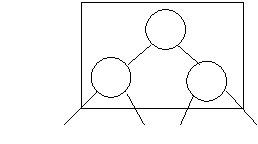
\includegraphics{Lecture35-Dinesh/figs/fig6.pdf}%
\end{picture}%
\setlength{\unitlength}{4144sp}%
%
\begingroup\makeatletter\ifx\SetFigFont\undefined%
\gdef\SetFigFont#1#2#3#4#5{%
  \reset@font\fontsize{#1}{#2pt}%
  \fontfamily{#3}\fontseries{#4}\fontshape{#5}%
  \selectfont}%
\fi\endgroup%
\begin{picture}(1968,1093)(2146,-2402)
\put(2161,-2311){\makebox(0,0)[lb]{\smash{{\SetFigFont{7}{8.4}{\familydefault}{\mddefault}{\updefault}{\color[rgb]{0,0,0}$f(1,x_2,\ldots,x_n)$}%
}}}}
\put(3466,-2356){\makebox(0,0)[lb]{\smash{{\SetFigFont{7}{8.4}{\familydefault}{\mddefault}{\updefault}{\color[rgb]{0,0,0}$\overline{x_1}$}%
}}}}
\put(3151,-2356){\makebox(0,0)[lb]{\smash{{\SetFigFont{7}{8.4}{\familydefault}{\mddefault}{\updefault}{\color[rgb]{0,0,0}$x_1$}%
}}}}
\put(3826,-2311){\makebox(0,0)[lb]{\smash{{\SetFigFont{7}{8.4}{\familydefault}{\mddefault}{\updefault}{\color[rgb]{0,0,0}$f(0,x_2,\ldots,x_n)$}%
}}}}
\put(3376,-1591){\makebox(0,0)[lb]{\smash{{\SetFigFont{7}{8.4}{\familydefault}{\mddefault}{\updefault}{\color[rgb]{0,0,0}$\lor$}%
}}}}
\put(3736,-1951){\makebox(0,0)[lb]{\smash{{\SetFigFont{7}{8.4}{\familydefault}{\mddefault}{\updefault}{\color[rgb]{0,0,0}$\lor$}%
}}}}
\put(2971,-1951){\makebox(0,0)[lb]{\smash{{\SetFigFont{7}{8.4}{\familydefault}{\mddefault}{\updefault}{\color[rgb]{0,0,0}$\lor$}%
}}}}
\end{picture}%

\caption{Circuit computing $f$}
\label{figure6}
\end{figure}
Hence $f(x_1,x_2,\ldots,x_n)$ can be expressed in the form of a recursive 
structure as, 
\begin{figure}[htp!]
\centering
\begin{picture}(0,0)%
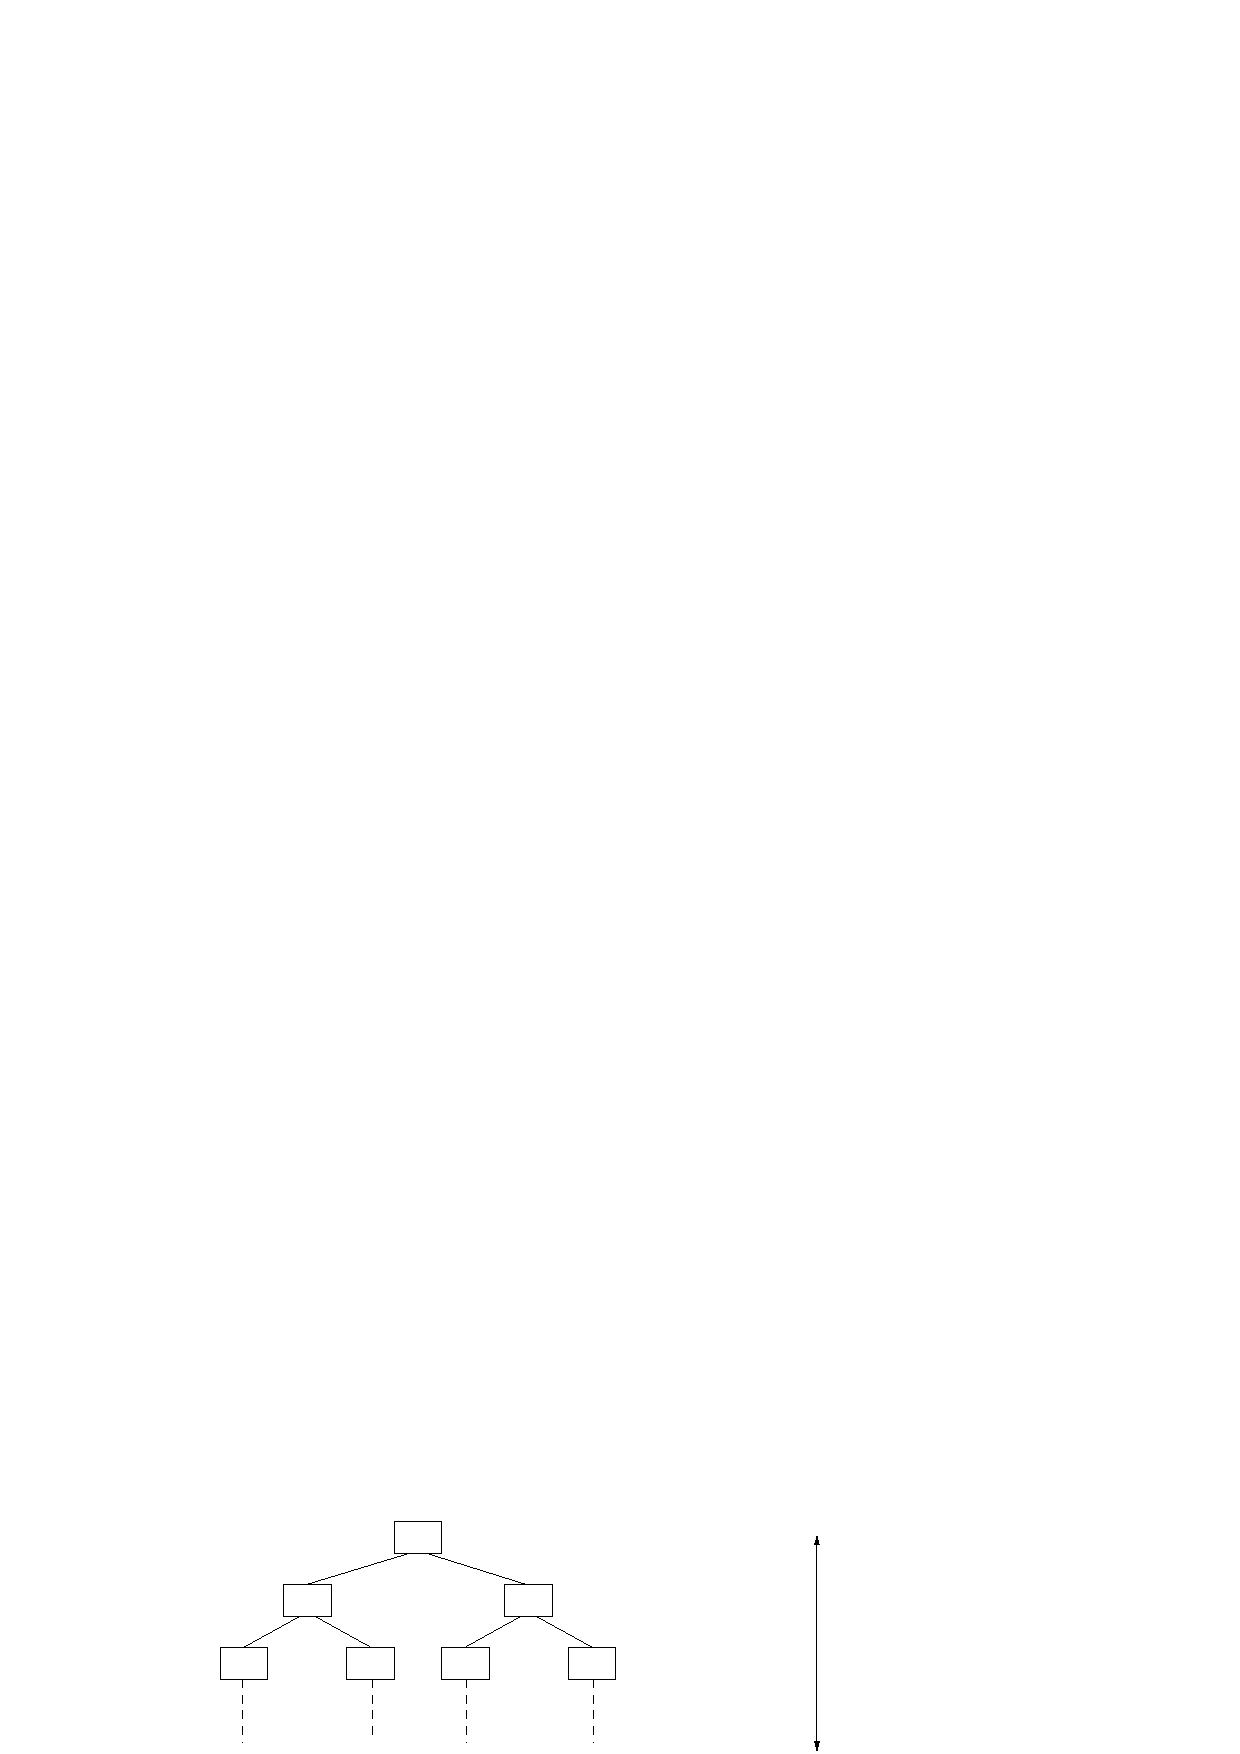
\includegraphics{Lecture35-Dinesh/figs/fig7.pdf}%
\end{picture}%
\setlength{\unitlength}{4144sp}%
%
\begingroup\makeatletter\ifx\SetFigFont\undefined%
\gdef\SetFigFont#1#2#3#4#5{%
  \reset@font\fontsize{#1}{#2pt}%
  \fontfamily{#3}\fontseries{#4}\fontshape{#5}%
  \selectfont}%
\fi\endgroup%
\begin{picture}(6266,1782)(-239,-2956)
\put(6012,-2029){\makebox(0,0)[lb]{\smash{{\SetFigFont{7}{8.4}{\familydefault}{\mddefault}{\updefault}{\color[rgb]{0,0,0}$n$}%
}}}}
\put(1971,-1836){\makebox(0,0)[lb]{\smash{{\SetFigFont{7}{8.4}{\familydefault}{\mddefault}{\updefault}{\color[rgb]{0,0,0}$x_2$}%
}}}}
\put(3657,-1836){\makebox(0,0)[lb]{\smash{{\SetFigFont{7}{8.4}{\familydefault}{\mddefault}{\updefault}{\color[rgb]{0,0,0}$x_2$}%
}}}}
\put(4138,-2317){\makebox(0,0)[lb]{\smash{{\SetFigFont{7}{8.4}{\familydefault}{\mddefault}{\updefault}{\color[rgb]{0,0,0}$x_3$}%
}}}}
\put(3175,-2317){\makebox(0,0)[lb]{\smash{{\SetFigFont{7}{8.4}{\familydefault}{\mddefault}{\updefault}{\color[rgb]{0,0,0}$x_3$}%
}}}}
\put(2453,-2317){\makebox(0,0)[lb]{\smash{{\SetFigFont{7}{8.4}{\familydefault}{\mddefault}{\updefault}{\color[rgb]{0,0,0}$x_3$}%
}}}}
\put(2815,-1354){\makebox(0,0)[lb]{\smash{{\SetFigFont{7}{8.4}{\familydefault}{\mddefault}{\updefault}{\color[rgb]{0,0,0}$x_1$}%
}}}}
\put(3271,-1354){\makebox(0,0)[lb]{\smash{{\SetFigFont{7}{8.4}{\familydefault}{\mddefault}{\updefault}{\color[rgb]{0,0,0}Computes $f(x_1,x_2,\ldots,x_n)$}%
}}}}
\put(4090,-1764){\makebox(0,0)[lb]{\smash{{\SetFigFont{7}{8.4}{\familydefault}{\mddefault}{\updefault}{\color[rgb]{0,0,0}Computes $f(1,x_2,\ldots,x_n)$}%
}}}}
\put(3513,-1546){\makebox(0,0)[lb]{\smash{{\SetFigFont{7}{8.4}{\familydefault}{\mddefault}{\updefault}{\color[rgb]{0,0,0}$x_1=1$}%
}}}}
\put(2044,-1546){\makebox(0,0)[lb]{\smash{{\SetFigFont{7}{8.4}{\familydefault}{\mddefault}{\updefault}{\color[rgb]{0,0,0}$x_1=0$}%
}}}}
\put(1490,-2317){\makebox(0,0)[lb]{\smash{{\SetFigFont{7}{8.4}{\familydefault}{\mddefault}{\updefault}{\color[rgb]{0,0,0}$x_3$}%
}}}}
\put(4478,-2311){\makebox(0,0)[lb]{\smash{{\SetFigFont{7}{8.4}{\familydefault}{\mddefault}{\updefault}{\color[rgb]{0,0,0}Computes $f(1,1,\ldots,x_n)$}%
}}}}
\put(-224,-2311){\makebox(0,0)[lb]{\smash{{\SetFigFont{7}{8.4}{\familydefault}{\mddefault}{\updefault}{\color[rgb]{0,0,0}Computes $f(0,0,x_3\ldots,x_n)$}%
}}}}
\put(316,-1861){\makebox(0,0)[lb]{\smash{{\SetFigFont{7}{8.4}{\familydefault}{\mddefault}{\updefault}{\color[rgb]{0,0,0}Computes $f(0,x_2,\ldots,x_n)$}%
}}}}
\end{picture}%

\caption{Complete circuit computing $f$}
\label{figure7}
\end{figure}
where each box represents the two $\land$ and one $\lor$ of 
figure~\ref{figure6}. 
Now, we can find the size of the circuit follows the recurrence 
\[S(n) =2S(n-1) + 6\]\[ S(2) = 1 \] where $6 = (1 - \land, 2 - \lor, 
\text{one } \neg \text{ of } \overline{x_1}, 
\text{ and } 0,1 \text{ inputs})$. Hence $S(n) = \frac{7}{4}2^n - 6 = O(2^n)$.
Note that this is a better bound than the bound from the trivial circuit. 
So the question is how much more can we improve ? How to make the circuit more 
compact ?
\begin{theorem}(Lupanov, 1952) An function on input defined on the complete
basis $\Omega = \{ \neg, \lor, \land\}$ of two input gates can be computed by a
 circuit of size $[1+o(1)]\frac{2^n}{n}$.
\end{theorem}
\begin{proof}
Observe that at the $k^{th}$ level (see figure~\ref{figure8}) for $0 < k \le n$ 
(where the bottom of the circuit is level 0) there are $k$ variables appearing
below it (All the $n-k$ variables above the $k^{th}$ level would have got
$0$ or $1$ assigned).
\begin{figure}[htp!]
\centering
\begin{picture}(0,0)%
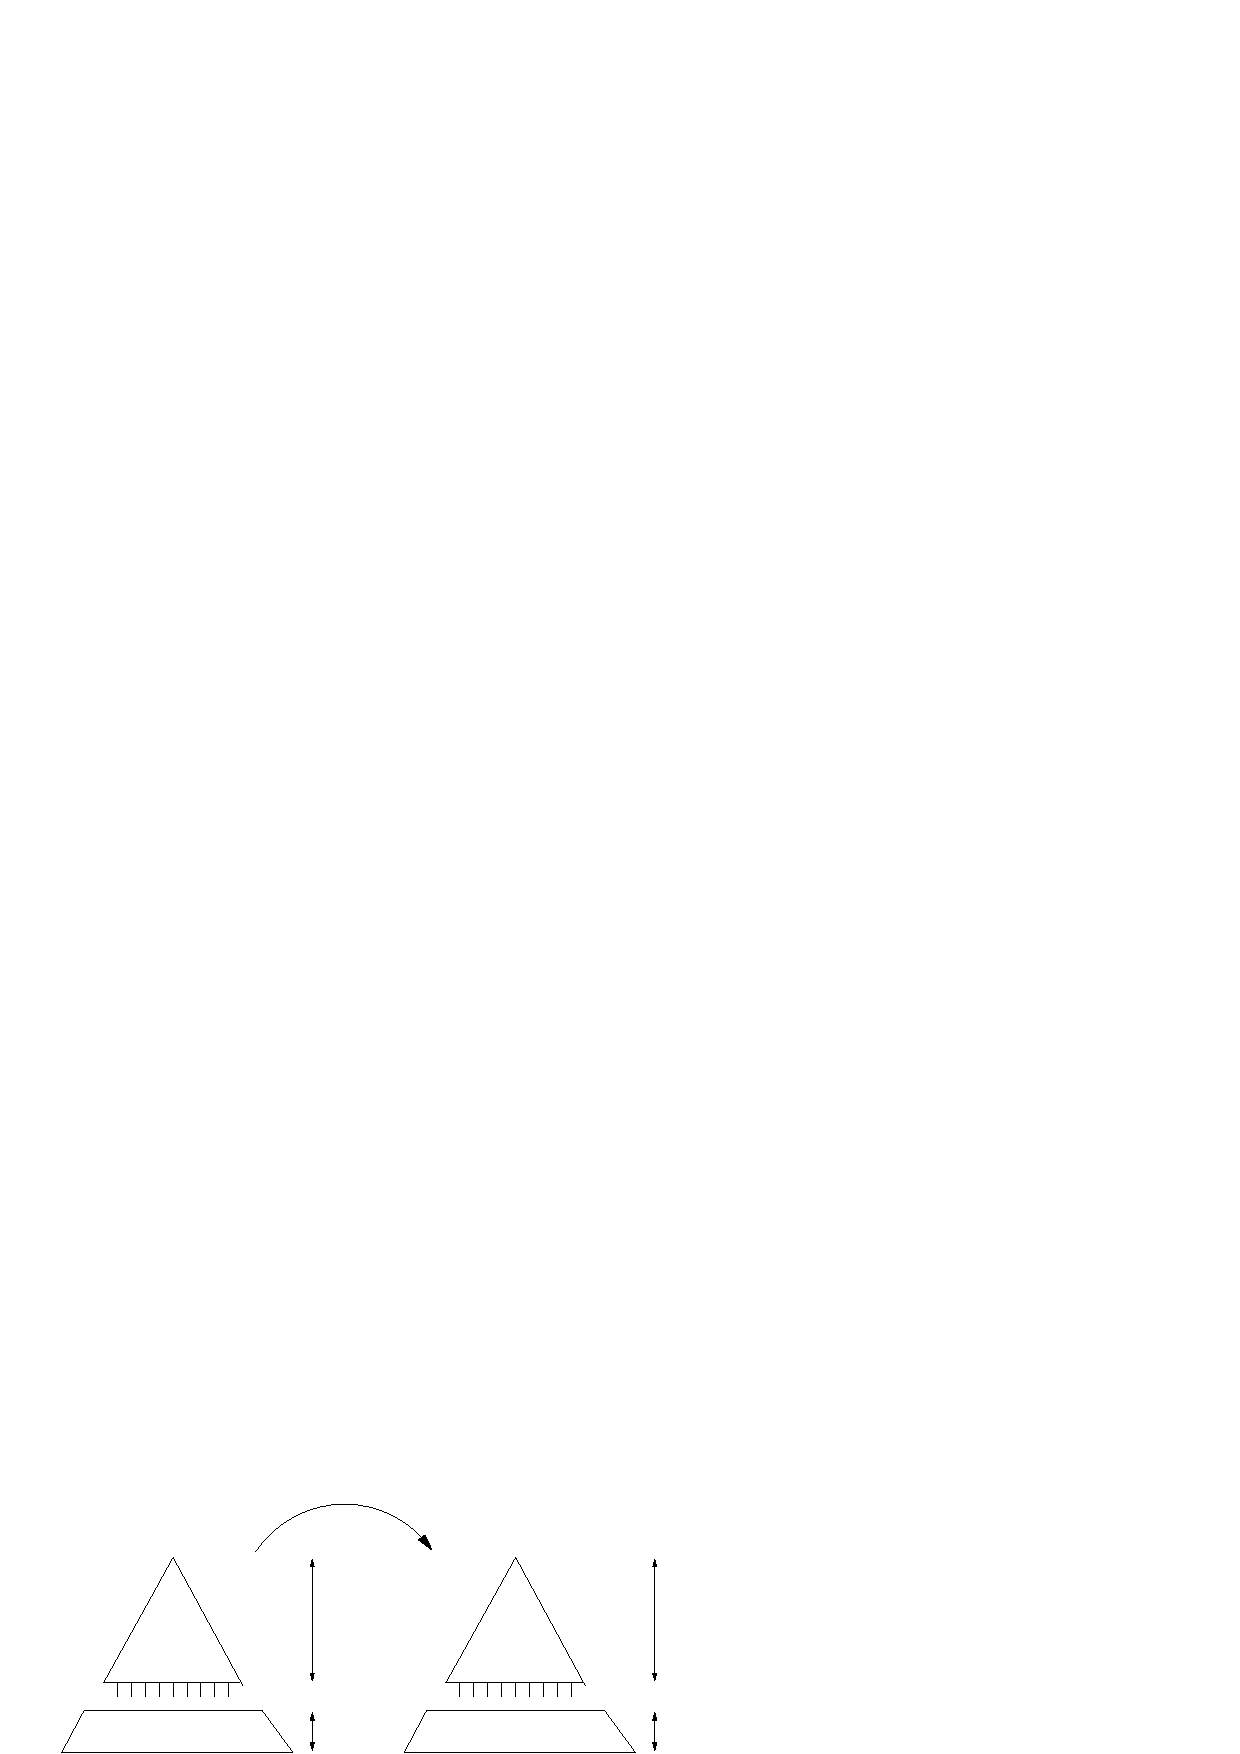
\includegraphics{Lecture35-Dinesh/figs/fig8.pdf}%
\end{picture}%
\setlength{\unitlength}{4144sp}%
%
\begingroup\makeatletter\ifx\SetFigFont\undefined%
\gdef\SetFigFont#1#2#3#4#5{%
  \reset@font\fontsize{#1}{#2pt}%
  \fontfamily{#3}\fontseries{#4}\fontshape{#5}%
  \selectfont}%
\fi\endgroup%
\begin{picture}(5068,1913)(2146,-2683)
\put(7178,-1716){\makebox(0,0)[lb]{\smash{{\SetFigFont{6}{7.2}{\familydefault}{\mddefault}{\updefault}{\color[rgb]{0,0,0}$n-k$}%
}}}}
\put(7199,-2501){\makebox(0,0)[lb]{\smash{{\SetFigFont{6}{7.2}{\familydefault}{\mddefault}{\updefault}{\color[rgb]{0,0,0}$k$}%
}}}}
\put(4568,-1716){\makebox(0,0)[lb]{\smash{{\SetFigFont{6}{7.2}{\familydefault}{\mddefault}{\updefault}{\color[rgb]{0,0,0}$n-k$}%
}}}}
\put(4590,-2501){\makebox(0,0)[lb]{\smash{{\SetFigFont{6}{7.2}{\familydefault}{\mddefault}{\updefault}{\color[rgb]{0,0,0}$k$}%
}}}}
\put(2999,-2565){\makebox(0,0)[lb]{\smash{{\SetFigFont{6}{7.2}{\familydefault}{\mddefault}{\updefault}{\color[rgb]{0,0,0}Dependent on $k$ inputs}%
}}}}
\put(2161,-2086){\makebox(0,0)[lb]{\smash{{\SetFigFont{6}{7.2}{\familydefault}{\mddefault}{\updefault}{\color[rgb]{0,0,0}$3.2^{n-k}$ gates}%
}}}}
\put(5851,-2446){\makebox(0,0)[lb]{\smash{{\SetFigFont{6}{7.2}{\familydefault}{\mddefault}{\updefault}{\color[rgb]{0,0,0}$A(k)$ gates }%
}}}}
\put(5626,-2626){\makebox(0,0)[lb]{\smash{{\SetFigFont{6}{7.2}{\familydefault}{\mddefault}{\updefault}{\color[rgb]{0,0,0}(All $2^{2^k}$ functions)}%
}}}}
\end{picture}%

\caption{Compacting of circuit}
\label{figure8}
\end{figure}

Also from our construction, it is clear that there are $3(2^{n-k})$ gates at
the $k^{th}$ level. Since circuits are DAGs the input to these gates can only
come from the $k$ variables. Also there can be $2^{2^k}$ distinct functions
computable using $k$ inputs. Now if $A(k)$ is the number of gates required to
realise these $2^{2^k}$ distinct functions then the $3(2^{n-k})$ gates can get
input from any of the $A(k)$ gates and if we have the case where $3(2^{n-k}) >
A(k)$ (after appropriately setting $k$), the result of computation can be
reused and compaction can be achieved. So unlike the earlier case where we
might have needed at least $3(2^{n-k})$ gates below the $k^{th}$ level, it now
suffices to generate all $2^{2^k}$ functions.

Now it remains to estimate $A(k)$. This function can be recursively
characterised as \[(x_k \land f_1(x_1,x_2,\ldots,x_{k-1}) \lor (\overline{x_k}
\land f_2(x_1,x_2,\ldots,x_{k-1})\] If we have the circuits computing all 
the $k-1$ input functions, we can construct circuits computing 
all of the $k$ input function using the recursive formulation.

Note that the total number of gates required to realise $2^{2^k}$ functions =
$ A(k) $ 
\begin{center} = (Gates required to realise $k$ variate functions from circuit
computing functions on $k-1$ variables) 

$+$ 

Number of gates required to realise all the $2^{2^{k-1}}$ functions.
\end{center}

The first term equals
\begin{align*}
= & \text{Total no. of $\land$ gates} + \text{Total no. of $\lor$ gates}  \\
= & (2^{2^{k-1}}) \times 2 +  (2^{2^{k-1}}) \times (2^{2^{k-1}}) 
&& [\text{Two $\land$ gates per $f$}] \\
& && [\text{Ways of choosing $f_1$, $f_2$}] 
\end{align*}
The second term is nothing but $A(k-1)$. Hence,
\begin{align*}
A(k) &=  A(k-1) + 2^{2^{k-1}} \times 2 + 2^{2^k} \\
A(0) &= 2 &&[\text{i.e. True or False}] 
\end{align*}
Note that this is nothing but the series summation
\begin{align*}
= & \sum_{i=1}^k (2^{2^i} + 2.2^{2^{i-1}}) + A(0) \\
= & \sum_{i=1}^k 2^{2^i} + \sum_{i=1}^k 2.2^{2^{i-1}} + A(0) \\
= & \sum_{i=0}^{k-1} 2^{2^i} + \sum_{i=0}^{k-1} 2.2^{2^i} + 2 + 2^{2^k} + A(0)
\\
= & 3\sum_{i=0}^{k-1} 2^{2^i} + 4 + 2^{2^k} \\
< &~3\sum_{i=0}^{k-1} 2^{2^{k-1}} + 2^{2^k} \\
= & 2^{2^k}+ 3k.2^{2^{k-1}} = 2^{2^k} \left ( 1 + \frac{3k}{2^{({2^k} -
2^{k-1})}}  \right )\\
\end{align*}
Hence $A(k) =  2^{2^k}(1+ o(1))$. Therefore total number of gates = $3.2^{n-k}
+ 2^{2^k}(1+o(1))$. Now to have $3.2^{n-k} > 2^{2^k}$, we choose $k = \log (n
- \log n)$ (verification of $k$ is left to the reader). 
Total number of gates is now
\begin{align*}
= & 3.\frac{2^n}{n-\log n} + \frac{2^n}{n}(1+o(1)) \\
= & \frac{2^n}{n} \left [ \frac{3}{1-\frac{\log n}{n}} + 1 + o(1)\right ] \\
\le & \frac{2^n}{n}(4 + o(1))
\end{align*}
This proves a bound which is almost as tight as the Lupanov's bound. Reducing
the constant from $4$ to $1$ requires more effort.
\end{proof}

